%% Report on S3-3HDM scalar decays and LFV Higgs rates.
%% Companion: derivations_03.tex (the derivation ledger, auto-generated by the notebook).
%% Source: research/thdm_s3/03_scalar_decays.ipynb
\documentclass[11pt,a4paper]{article}
\usepackage[T1]{fontenc}
\usepackage[utf8]{inputenc}
\usepackage{amsmath,amssymb}
\usepackage{graphicx}
\usepackage{booktabs}
\usepackage[margin=2.4cm]{geometry}
\usepackage[colorlinks=true,linkcolor=blue,citecolor=blue,urlcolor=blue]{hyperref}
\setlength{\parindent}{0pt}
\setlength{\parskip}{0.6em}

\title{Scalar decays and LFV Higgs rates in the $S_3$-symmetric 3HDM:\\
a gauge-phobic state for every $\delta$, and an LFV bound\\
on the lepton sector rather than the scalars}
\author{M. Zeleny-Mora\\[2pt]
\small Instituto de Física, Universidad Nacional Autónoma de México}
\date{\today}

\begin{document}
\maketitle

\begin{abstract}
\noindent
I have turned the LFV couplings of our draft \cite{LFVHD} into branching ratios, over every
viable point of the scalar scan. The CP-even basis $R_S=R_AR_H(\delta)$ is kept at
\emph{general} $\delta$, so the draft's scenarios A and B appear only as limits. Three
structural results follow. First, $h_0$ is gauge-phobic \emph{exactly, for every} $\delta$:
$g_{h_0VV}=0$ identically, while its LFV couplings do not depend on $\delta$ at all.
Second, $\delta$ is not a free dial: the quartics predict it at each point, and
$|\delta|\le0.32$ over the viable set. Third, the draft's Scenario-C relations, printed
with ``$\approx$'', are exact. Phenomenologically, $\mathcal B(h\to\mu\tau)$ from the
SM-like state exceeds the CMS limit \cite{CMS21} in 18\% of entries, and that fraction is
carried almost entirely by the lepton-sector parameter $\mu_3^\ell$. LFV data therefore
bound $\mu_3^\ell$, not the scalar sector. $\mathcal B(h\to\tau e)$ vanishes to machine
precision, for the same reason that exact $S_3$ forces $V_{us}=0$. Two library gaps were
closed along the way: VSS decays and the spin-0 $\gamma\gamma$ form factor.
\end{abstract}

\section{Summary}

Everything below comes from \texttt{research/thdm\_s3/03\_scalar\_decays.ipynb}. It
registers the physical basis on the \texttt{feynlag} model, extracts every Feynman rule from
the Lagrangian, and runs the decay engine over the 1964 viable points of the scalar scan.

\begin{enumerate}\itemsep2pt
\item \textbf{$h_0$ is gauge-phobic for any $\delta$}, and the other two CP-even states
share the SM coupling as $\cos\delta$, $\sin\delta$ (\S\ref{sec:gauge}).
\item \textbf{$\delta$ is predicted, and $\delta=-\psi$}, not the $\alpha-\theta_v$ I first
used. That earlier formula mis-assigned the couplings; it is corrected here and in every
downstream number (\S\ref{sec:delta}).
\item \textbf{The draft's Scenario-C relations are exact}, and $Q_2$ (the $h_0$ couplings)
does not depend on $\delta$ (\S\ref{sec:scenarioC}).
\item \textbf{LFV rates}: $h\to\mu\tau$ constrains $\mu_3^\ell$; $h\to\tau e$ is structurally
zero (\S\ref{sec:lfv}). This is the main phenomenological result.
\item \textbf{Two library gaps closed}: VSS decays ($A\to Zh$, $H^\pm\to W^\pm h$) and the
spin-0 form factor $A_0$ for charged-Higgs $\gamma\gamma$ loops (\S\ref{sec:library}).
\end{enumerate}

\section{The physical basis}

Five rotations are registered on the model: the three scalar rotations ($R_S=R_AR_H(\delta)$
for the CP-even states, $R_A$ for the CP-odd and charged), plus the Weinberg and
charged-current rotations. Every vertex below is therefore extracted from the Lagrangian in
the physical basis rather than written down. $R_H(\delta)$ acts only in the $1$--$3$ plane,
and $R_S$ is orthogonal for any $\delta$.

\section{The gauge couplings at general $\delta$}
\label{sec:gauge}

$R_A$'s first column is the unit vacuum direction $\hat n$ \cite{LFVHD}. The $hVV$ couplings
come out as
\[
g_{h_iVV}=g^{\rm SM}\,\big(R_S^{\mathsf T}\hat n\big)_i
=g^{\rm SM}\,(\cos\delta,\ 0,\ \sin\delta),
\qquad
\sum_i g_{h_iVV}^2=\big(g^{\rm SM}\big)^2 ,
\]
for $W$ and $Z$ alike. The SM reference $g^{\rm SM}=ig_wm_W$ is read off the $\delta\to0$
limit, not typed in. The middle zero is $h_0$: $R_H$ never touches it, so its column of
$R_S$ is $R_A$'s middle column, which is orthogonal to $\hat n$. The zero survives at a
generic vacuum angle, so it is orthogonality, not the $\sqrt3$ alignment.
\cite{GomezBock21}'s scenarios are the limits:

\begin{center}
\begin{tabular}{lccc}
\toprule
scenario & $g_{h_1VV}/g^{\rm SM}$ & $g_{h_2VV}/g^{\rm SM}$ & $g_{h_0VV}$\\
\midrule
A ($\delta\to0$) & $1$ & $0$ & $0$\\
B ($\delta\to\pi/2$) & $0$ & $1$ & $0$\\
C (general) & $\cos\delta$ & $\sin\delta$ & $0$\\
\bottomrule
\end{tabular}
\end{center}

\section{$\delta$ is predicted, and it is $-\psi$}
\label{sec:delta}

$\delta$ is fixed by the residual CP-even $2\times2$ block, whose angle $\psi$ the
scalar-sector code computes at every point. \textbf{A correction I owe you here:} I first
used $\delta=\alpha-\theta_v$. The correct relation is $\delta=-\psi$, for two reasons.
\begin{itemize}\itemsep1pt
\item $R_H$'s $(0,2)$ block is $\mathrm{rot}(\delta)$, while the library's 2×2 solver returns
the angle that diagonalises the transpose, which accounts for the sign.
\item $R_A(\phi,\theta_v)R_H(\delta)=R_A(\phi,\theta_v+\delta)$ identically. So the draft's
total angle is $\alpha=\theta_v+\delta$, and there is no $\theta_v$ to subtract from a block
angle that is already measured from the geometric basis.
\end{itemize}
The old formula left $R_S^{\mathsf T}M_SR_S$ off-diagonal at the $10^5$ level and
mis-assigned the couplings: at benchmark point~0 it gave $\cos^2\delta=0.55$ where the true
value is $0.995$. Every number in this report uses $\delta=-\psi$, which is checked against
the stored scan values to $4\times10^{-6}$ (the $\lambda$ rounding).

\begin{figure}[h]
\centering
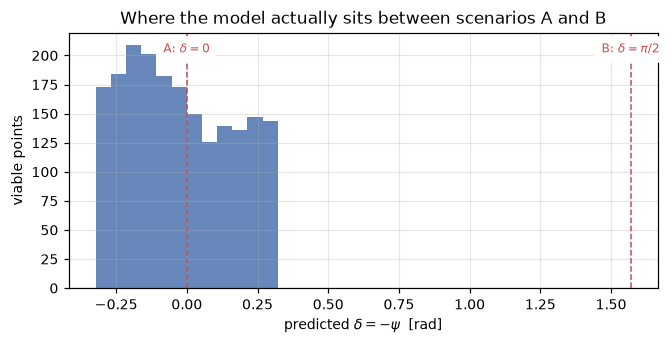
\includegraphics[width=0.78\textwidth]{figures/decays_delta_scenarios.png}
\caption{The predicted $\delta=-\psi$ over the 1964 viable points. The model sits near
scenario A, and never near B.}
\label{fig:delta}
\end{figure}

Over the viable set $\delta\in[-0.322,\,0.321]$ and $\cos^2\delta\in[0.900,\,1.000]$. Because
$\psi=\tfrac12\arctan(\cdot)\in(-\pi/4,\pi/4)$, $\cos^2\delta\ge\tfrac12$ always. $h_1$ is
therefore by convention the state with the larger $VV$ coupling, and scenario B is a
symbolic limit that the scan cannot reach. The SM-like state is $H_2$ at every listed
benchmark point.

\section{The draft's Scenario-C relations are exact}
\label{sec:scenarioC}

\cite{LFVHD} prints the Scenario-C LFV couplings with ``$\approx$''. They hold identically
for all $\delta$, because $Q_i$ is linear in the columns of $R_S=R_AR_H(\delta)$:
$Q_1(C)$ and $Q_3(C)$ are exact rotations of $Q_1(A)$ and $Q_3(A)$, and
\[
Q_2(C)=Q_2(A)\qquad\text{exactly.}
\]
Together with \S\ref{sec:gauge}, this makes $h_0$ the state with no $VV$ coupling and
$\delta$-independent lepton couplings. It is the one CP-even state whose LFV decays the
alignment cannot suppress.

\section{LFV rates against the CMS limits}
\label{sec:lfv}

With $\mathcal L\supset-h\,\bar\ell_aQ_{ab}P_R\ell_b+\text{h.c.}$, the width in the
$m_\ell\ll m_h$ limit is
\[
\Gamma(h\to\ell_a\bar\ell_b+\bar\ell_a\ell_b)=\frac{m_h}{8\pi}\big(|Q_{ab}|^2+|Q_{ba}|^2\big),
\]
which the engine reproduces from the extracted FFS vertices. Branching ratios are quoted
against the measured total width $\Gamma_h=4.1$~MeV \cite{PDG}. That is the standard
convention in LFV searches, and the honest one here, since the quark Yukawas are not in this
build.

The lepton Yukawas are fixed by the three masses up to one free parameter, $\mu_3^\ell$. The
inversion is verified along the whole $\mu_3$ range: the singular values of $M_\ell$ equal
$(m_e,m_\mu,m_\tau)$ to $10^{-9}$, and a 1\% change in $\mu_4$ breaks it. The rates are
evaluated at $\mu_3^\ell=0.5,\ 0.9,\ 1.4$~GeV over all 1964 points, giving 23\,568
(point, $\mu_3$, state, channel) entries.

\begin{center}
\begin{tabular}{llrrr}
\toprule
state & channel & median $\mathcal B$ & max $\mathcal B$ & over the limit\\
\midrule
SM-like & $\mu\tau$ & $1.7\times10^{-4}$ & $0.14$ & $1070/5892$ (18\%)\\
SM-like & $e\tau$ & $5.7\times10^{-35}$ & $1.3\times10^{-33}$ & $0/5892$\\
$h_0$ (gauge-phobic) & $\mu\tau$ & $8.8\times10^{-3}$ & $9.1^{\,*}$ & $4760/5892$ (81\%)\\
$h_0$ (gauge-phobic) & $e\tau$ & $1.5\times10^{-34}$ & $1.9\times10^{-31}$ & $0/5892$\\
\bottomrule
\end{tabular}

{\small CMS limits \cite{CMS21}: $\mathcal B(h\to\mu\tau)<0.15\%$, $\mathcal B(h\to e\tau)<0.22\%$
at 95\% CL. $^*$For $h_0$ the ``branching ratio'' is a ratio to the SM-like width, not its
own; see open question~1.}
\end{center}

\paragraph{$h\to\mu\tau$ bounds $\mu_3^\ell$, not the scalar sector.} The SM-like
over-the-limit fraction is carried almost entirely by $\mu_3^\ell$:

\begin{center}
\begin{tabular}{lccc}
\toprule
$\mu_3^\ell$ [GeV] & $0.5$ & $0.9$ & $1.4$\\
\midrule
SM-like $\mathcal B(h\to\mu\tau)$, median & $3.9\times10^{-5}$ & $2.5\times10^{-4}$ & $1.4\times10^{-3}$\\
fraction above $0.15\%$ & $0.3\%$ & $6.4\%$ & $48\%$\\
\bottomrule
\end{tabular}
\end{center}

The median point over the full scan sits a factor of about~9 \emph{below} the limit. (An
earlier version of this result said the model ``generically overshoots''. That was computed
with the wrong $\delta$ \emph{and} before the coupling cut on the scalar scan, which together
moved the SM-like median from $1.9\times10^{-3}$ to $1.7\times10^{-4}$.)

\begin{figure}[h]
\centering
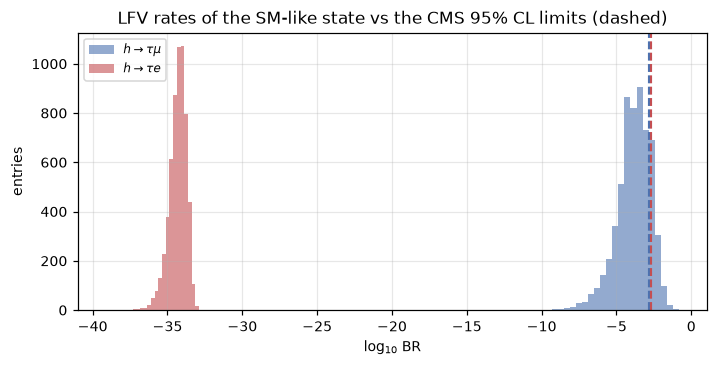
\includegraphics[width=0.80\textwidth]{figures/decays_lfv_limits.png}
\caption{LFV branching ratios of the SM-like state over all points and $\mu_3^\ell$ values,
against the CMS 95\% CL limits (dashed). $h\to\tau\mu$ straddles the limit; $h\to\tau e$ sits
near $10^{-34}$, which is zero to machine precision.}
\label{fig:lfv}
\end{figure}

\paragraph{$h\to\tau e$ is structurally absent.} The largest value anywhere in the scan is
$1.9\times10^{-31}$. That is not a small number, it is zero. $O_{12}$ separates the electron
exactly at the aligned vacuum, so no $e$--$\tau$ entry can be generated. This is the same
first-generation decoupling that forces $V_{us}=0$ in the quark sector (companion fermion
report). The exact-$S_3$ vacuum ties the quark and lepton flavour structures together, and
the two calculations see the same fact from opposite ends.

\section{Two library gaps closed}
\label{sec:library}

\paragraph{VSS decays.} $A_i\to Zh_j$ and $H_i^\pm\to W^\pm h_j$ go through derivative
couplings $gV^\mu(S\partial_\mu S'-S'\partial_\mu S)$, which the decay engine used to
refuse. Every benchmark point has such channels open, and they are gauge-strength, so
omitting them would have made the heavy-state branching ratios wrong, not just incomplete.
They are now squared:
\[
\Gamma(S\to VS')=\frac{|c|^2\,\lambda^{3/2}(m_S^2,m_V^2,m_{S'}^2)}{16\pi\,m_S^3\,m_V^2},
\]
verified against that closed form and against an independent explicit polarization sum.
The model has three $A\to Zh$ vertices ($A_1Zh_0$, $A_2Zh_1$, $A_2Zh_2$) and three
$H^\pm\to W^\pm h$ vertices with the same pattern.

\paragraph{The spin-0 $\gamma\gamma$ form factor.} A 3HDM has two charged Higgses in the
$h\to\gamma\gamma$ loop, which needs
\[
A_0(\tau)=\frac{\tau-f(\tau)}{\tau^2},\qquad\tau=\frac{m_h^2}{4m^2}.
\]
Its sign is not copied but forced. \cite{ChakrabortiEtAl21} Eq.~(28) gives $F_W\to+7$,
$F_t\to-4/3$, $F^+\to+1/3$. Since the library has $A_1=-F_W$ and $A_{1/2}=-F_t$
\cite{Djouadi08}, consistency requires $A_0=-F^+\to-1/3$. All three form factors reach their
decoupling limits ($+4/3$, $-7$, $-1/3$), and the SM width comes out at
$\Gamma(h\to\gamma\gamma)=9.195$~keV against PDG's $\approx9.3$~keV.

\begin{figure}[h]
\centering
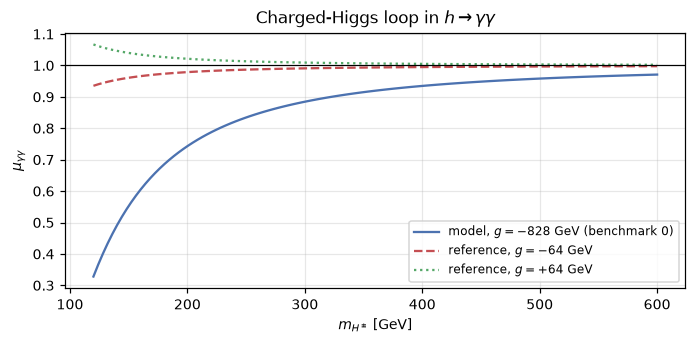
\includegraphics[width=0.78\textwidth]{figures/decays_gammagamma.png}
\caption{The charged-Higgs contribution to $\mu_{\gamma\gamma}$ against $m_{H^\pm}$. Solid:
this model's largest trilinear at benchmark point~0, $g(h_1H_1^+H_1^-)=-828$~GeV.
Dashed and dotted: reference couplings $\mp64$~GeV. The loop decouples as $m_{H^\pm}\to\infty$,
as it must.}
\label{fig:gg}
\end{figure}

\clearpage
\section{Open questions, and what would help}

\begin{enumerate}\itemsep4pt
\item \textbf{The $h_0$ ``branching ratios'' are ratios to the SM-like total width.} That is
the only width this build has, and it is not $h_0$'s own. These numbers are rate ratios,
not branching fractions: 11 of the 5892 $h_0$ entries exceed 1, which shows the artefact
rather than a new problem. The SM-like numbers are unaffected.
\item \textbf{The quark channels are absent}, so the total width is taken from experiment
and there are no $b\bar b$/$c\bar c$ branching ratios. This is deliberate: the exact-$S_3$
quark sector is excluded ($V_{us}=0$), and fitting it would mean quoting rates from a sector
known to be wrong. The heavy-state branching ratios ($A_{1,2}$, $H^\pm$) need the same quark
input to be complete.
\item \textbf{Redo the rates in the soft-broken vacuum.} That is where the quark sector works.
But there the CP-even mixing is a full $3\times3$ with no gauge-phobic state, so the single
angle $\delta$ no longer applies (companion soft-vacuum report). The couplings have to be
regenerated from the stored mixing matrices.
\item \textbf{$Z\gamma$} would need a two-argument charged-scalar form factor, the analogue of
$A_0$. Untouched.
\item \textbf{$\mu_3^\ell$} is scanned rather than fixed. Is there a principled way to fix
it, for example from neutrino-sector input, or should the LFV bound on it be the quoted
result?
\end{enumerate}

\appendix
\section{The derivation ledger}

The full typeset version is the companion document \texttt{derivations\_03.tex}; in
summary:

\begin{center}
\begin{tabular}{p{0.30\textwidth}p{0.13\textwidth}p{0.47\textwidth}}
\toprule
claim & status & independent checks\\
\midrule
$g_{h_iVV}=g^{\rm SM}(\cos\delta,0,\sin\delta)$, with the sum rule & derived &
$R_A$'s first column verified to be $\hat n$; SM reference read off the $\delta\to0$ limit;
$W$ and $Z$ agree; the zero survives a generic vacuum angle\\
\addlinespace
$\mathrm{lepton\_mus}(\mu_3)$ inverts the mass relations & derived &
singular values match the PDG masses to $10^{-9}$ across the whole $\mu_3$ scan; the Yukawas
genuinely vary; a 1\% change in $\mu_4$ breaks it\\
\addlinespace
$A_{1/2}$, $A_1$, $A_0$ and the LFV width & \textbf{imported} \cite{Djouadi08,ChakrabortiEtAl21} &
decoupling limits $4/3$, $-7$, $-1/3$; the SM diphoton width is reproduced\\
\bottomrule
\end{tabular}
\end{center}

\begin{thebibliography}{9}

\bibitem{LFVHD} M.~Zeleny-Mora, M.~Mondragón and T.~A.~Valencia-Pérez,
\emph{Exploring LFV Higgs decays in the Three Higgs Doublet Model}, draft
(\texttt{paper\_lfvhd/LFVHD\_3HDMS3.tex}).

\bibitem{GomezBock21} M.~Gómez-Bock, M.~Mondragón and A.~Pérez-Martínez,
\emph{Scalar and gauge sectors in the 3-Higgs Doublet Model under the $S_3$-symmetry},
Eur.\ Phys.\ J.\ C \textbf{81}, 942 (2021),
\href{https://arxiv.org/abs/2102.02800}{arXiv:2102.02800},
\href{https://doi.org/10.1140/epjc/s10052-021-09731-3}{doi:10.1140/epjc/s10052-021-09731-3}.

\bibitem{CMS21} CMS Collaboration,
\emph{Search for lepton-flavor violating decays of the Higgs boson in the $\mu\tau$ and
$e\tau$ final states in pp collisions at $\sqrt s=13$~TeV},
Phys.\ Rev.\ D \textbf{104}, 032013 (2021),
\href{https://arxiv.org/abs/2105.03007}{arXiv:2105.03007},
\href{https://doi.org/10.1103/PhysRevD.104.032013}{doi:10.1103/PhysRevD.104.032013}.

\bibitem{ChakrabortiEtAl21} M.~Chakraborti, D.~Das, M.~Levy, S.~Mukherjee and I.~Saha,
\emph{Prospects of light charged scalars in a three Higgs doublet model with $Z_3$
symmetry}, \href{https://arxiv.org/abs/2104.08146}{arXiv:2104.08146}.

\bibitem{Djouadi08} A.~Djouadi,
\emph{The anatomy of electroweak symmetry breaking. I},
Phys.\ Rept.\ \textbf{457}, 1 (2008),
\href{https://arxiv.org/abs/hep-ph/0503172}{hep-ph/0503172}.

\bibitem{PDG} S.~Navas \emph{et al.} (Particle Data Group),
\emph{Review of Particle Physics}, Phys.\ Rev.\ D \textbf{110}, 030001 (2024),
\href{https://doi.org/10.1103/PhysRevD.110.030001}{doi:10.1103/PhysRevD.110.030001}.

\end{thebibliography}

\end{document}
